\documentclass[tikz, border=4pt]{standalone}
% Shared preamble for the qpo_*.tex query plan figures.
\usepackage[T1]{fontenc}
\usepackage{lmodern}
\usetikzlibrary{arrows.meta, positioning, fit, backgrounds, calc}

\definecolor{accent}{HTML}{2F5D8C}
\definecolor{groupfill}{HTML}{EEF3F8}
\definecolor{taskfill}{HTML}{FFFFFF}
\definecolor{note}{HTML}{555555}
\definecolor{hot}{HTML}{C0561B}
\definecolor{hotfill}{HTML}{FCEBDD}

\newcommand{\sub}{\tiny\color{note}}
\newcommand{\hsub}{\tiny\color{hot}}

\tikzset{
    every picture/.style={font=\sffamily\scriptsize, node distance=4mm},
    op/.style={draw=accent, fill=taskfill, rounded corners=2pt, line width=0.6pt,
               minimum width=30mm, minimum height=7mm, align=center, inner sep=2pt},
    tbl/.style={op, fill=groupfill},
    small/.style={minimum width=18mm},
    hot/.style={draw=hot, fill=hotfill, line width=1pt},
    flow/.style={-{Stealth[length=2mm]}, accent, line width=0.7pt},
    hotflow/.style={flow, color=hot, line width=0.9pt},
    panel/.style={draw=accent, dashed, rounded corners=4pt, line width=0.6pt, inner sep=3mm},
    lbl/.style={font=\sffamily\scriptsize\bfseries, text=accent},
    callout/.style={font=\sffamily\tiny, text=hot, align=left},
}

\begin{document}
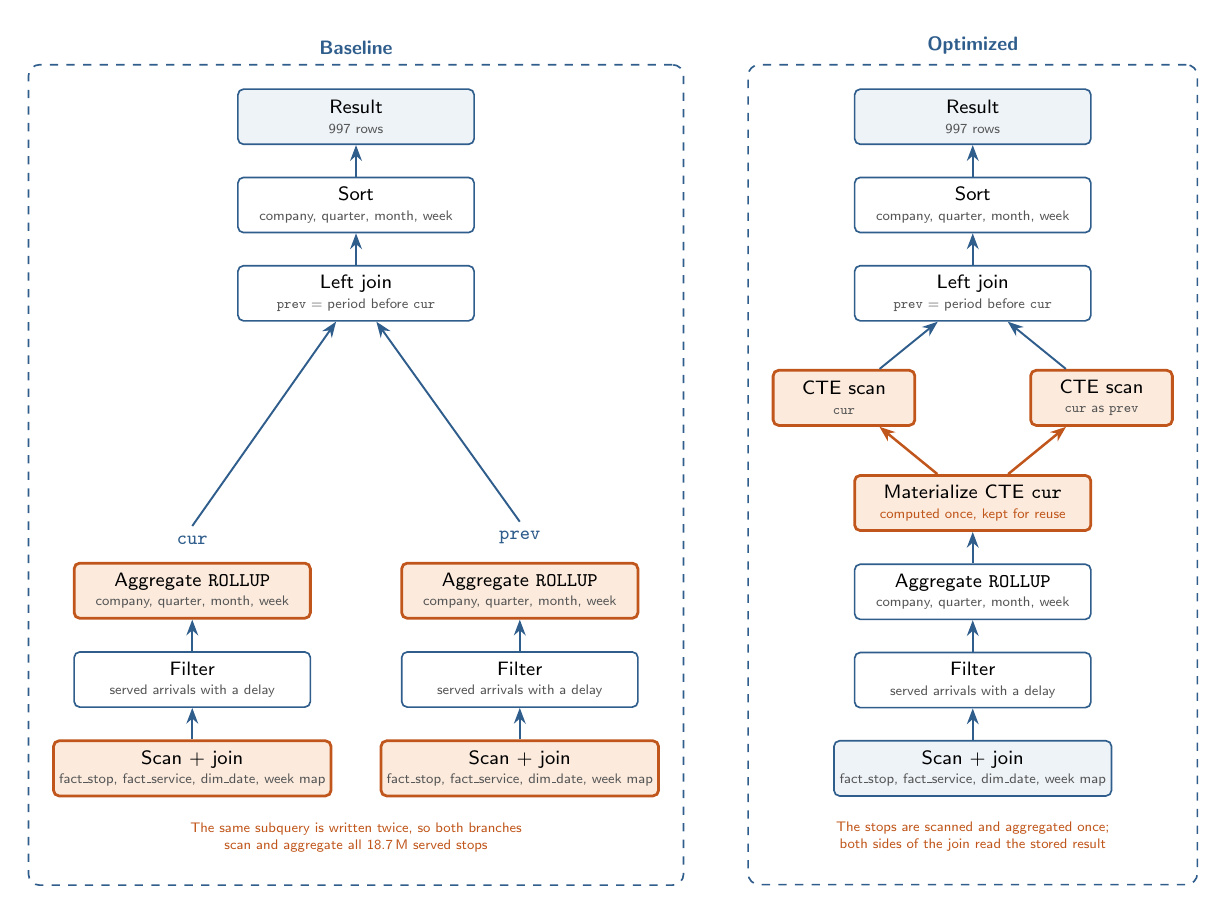
\begin{tikzpicture}

% ---------------- Baseline ----------------
\node[tbl, hot] (bs1) {Scan + join\\[-1pt]{\sub fact\_stop, fact\_service, dim\_date, week map}};
\node[op, above=of bs1] (bf1) {Filter\\[-1pt]{\sub served arrivals with a delay}};
\node[op, hot, above=of bf1] (ba1) {Aggregate \texttt{ROLLUP}\\[-1pt]{\sub company, quarter, month, week}};
\node[lbl, above=1mm of ba1] (bc1) {\texttt{cur}};

\node[tbl, hot, right=6mm of bs1] (bs2) {Scan + join\\[-1pt]{\sub fact\_stop, fact\_service, dim\_date, week map}};
\node[op, above=of bs2] (bf2) {Filter\\[-1pt]{\sub served arrivals with a delay}};
\node[op, hot, above=of bf2] (ba2) {Aggregate \texttt{ROLLUP}\\[-1pt]{\sub company, quarter, month, week}};
\node[lbl, above=1mm of ba2] (bc2) {\texttt{prev}};

\draw[flow] (bs1) -- (bf1);
\draw[flow] (bf1) -- (ba1);
\draw[flow] (bs2) -- (bf2);
\draw[flow] (bf2) -- (ba2);

% ---------------- Optimized ----------------
\node[tbl, right=22mm of bs2] (os) {Scan + join\\[-1pt]{\sub fact\_stop, fact\_service, dim\_date, week map}};
\node[op, above=of os] (of) {Filter\\[-1pt]{\sub served arrivals with a delay}};
\node[op, above=of of] (oa) {Aggregate \texttt{ROLLUP}\\[-1pt]{\sub company, quarter, month, week}};
\node[op, hot, above=of oa] (om) {Materialize CTE \texttt{cur}\\[-1pt]{\hsub computed once, kept for reuse}};

\node[op, hot, small, above left=6mm and -8mm of om] (oc1) {CTE scan\\[-1pt]{\sub \texttt{cur}}};
\node[op, hot, small, above right=6mm and -8mm of om] (oc2) {CTE scan\\[-1pt]{\sub \texttt{cur} as \texttt{prev}}};

\node[op, above=6mm of $(oc1.north)!0.5!(oc2.north)$] (oj) {Left join\\[-1pt]{\sub \texttt{prev} = period before \texttt{cur}}};
\node[op, above=of oj] (oo) {Sort\\[-1pt]{\sub company, quarter, month, week}};
\node[op, above=of oo, fill=groupfill] (or) {Result\\[-1pt]{\sub 997 rows}};

\draw[flow] (os) -- (of);
\draw[flow] (of) -- (oa);
\draw[flow] (oa) -- (om);
\draw[hotflow] (om) -- (oc1);
\draw[hotflow] (om) -- (oc2);
\draw[flow] (oc1) -- (oj);
\draw[flow] (oc2) -- (oj);
\draw[flow] (oj) -- (oo);
\draw[flow] (oo) -- (or);

\node[callout, below=2mm of os, align=center] (onote)
    {The stops are scanned and aggregated once;\\both sides of the join read the stored result};

\begin{scope}[on background layer]
  \node[panel, fit=(os)(or)(oc1)(oc2)(onote)] (opp) {};
\end{scope}
\node[lbl, anchor=south] at (opp.north) {Optimized};

% ---------------- Baseline top, aligned with the optimized side ----------------
\coordinate (bmid) at ($(ba1)!0.5!(ba2)$);
\node[op] (bj) at (bmid |- oj) {Left join\\[-1pt]{\sub \texttt{prev} = period before \texttt{cur}}};
\node[op, above=of bj] (bo) {Sort\\[-1pt]{\sub company, quarter, month, week}};
\node[op, above=of bo, fill=groupfill] (br) {Result\\[-1pt]{\sub 997 rows}};

\draw[flow] (bc1.north) -- (bj);
\draw[flow] (bc2.north) -- (bj);
\draw[flow] (bj) -- (bo);
\draw[flow] (bo) -- (br);

\node[callout, below=2mm of $(bs1.south)!0.5!(bs2.south)$, align=center] (bnote)
    {The same subquery is written twice, so both branches\\scan and aggregate all 18.7\,M served stops};

\begin{scope}[on background layer]
  \node[panel, fit=(bs1)(bs2)(br)(bnote)] (bp) {};
\end{scope}
\node[lbl, anchor=south] at (bp.north) {Baseline};

\end{tikzpicture}
\end{document}
